\documentclass[draft,linenumbers]{agujournal2018}
\documentclass{article}
\usepackage{amsmath}
\usepackage{amssymb}

\usepackage{subfigure}
\usepackage[colorinlistoftodos]{todonotes}
\usepackage[utf8]{inputenc}
%\usepackage{apacite}
%\usepackage{url} % should fix any errors with URLs in refs.
%\usepackage{subfig}
%\usepackage{xcolor}
%\usepackage[colorlinks]{hyperref}
%\usepackage{subfloat}
%\usepackage{subcaption}
%\usepackage[demo]{graphicx}

\draftfalse

%\journalname{Space Weather}

% Journal options
% https://docs.google.com/document/d/1hGGISS5dM__oSUb8JVXcjPFPBdVrGD_LNnkflubR6xw/edit

\newcommand{\citeay}[1]{%
\citeauthor{#1}, \citeyear{#1}%
}

\begin{document}

\title{The Magnetotelluric Impedance at Middelpos, South Africa}

\authors{R.S. Weigel\affil{1} and P.J. Cilliers\affil{2}}

\affiliation{1}{Space Weather Lab, George Mason University, 4400 University Drive, Fairfax VA 22030}
\affiliation{2}{South African National Space Agency, Hospital Street, Hermanus, 7200}

\correspondingauthor{R.S. Weigel}{rweigel@gmu.edu}

%\begin{keypoints}
%\item 
%\item 
%\item 
%\end{keypoints}

\begin{abstract}
From 2012-07-12 through 2012-11-07 (119 days), a magnetotelluric (MT) instrument made continuous 1-second recordings at Middelpos, a South Africa site. Two methods were used to compute the surface impedance transfer function (TF): (1) 119 TFs were computed and averaged using non--overlapping one-day segments, and (2) One TF was computed using the full 119-day segment. The error bars were calculated using parametric formulas that assume a known distribution of errors and a bootstrap method. A frequency domain quality metric, the signal--to--prediction error ($\text{SE}$), was calculated to assess the quality of predictions of the electric field from the computed TFs. The computed TFs have significant off-diagonal components, suggesting a complex ground conductivity structure. The SE is greater than one only in the range of 1--minute to 6--hours for the $E_x$--related terms and 1--minute to 1--hour for $E_y$--related terms. We also find differences in the transfer functions computed in two ways that are inconsistent with the error bars.
\end{abstract}

\section{Introduction}

The surface impedance of the Earth under a power line is an essential parameter in deriving the geomagnetically induced currents (GICs) in the power line from the measured or predicted geomagnetic field. The surface impedance is also the starting point for estimating the ground conductivity structure \cite{Simpson2005}. The surface impedance links the estimated electric field to the geomagnetic field. The surface impedance is typically derived from magnetotelluric (MT) measurements which combine co-located 3-axis magnetic field measurements with 2-axis horizontal electric field measurements (\cite{Naido2012}, \cite{Simpson2005}). The electric field (E-field) and magnetic field (B-field) are not independent of each other but are linked by a transfer function derived from Maxwell’s equations (\cite{Vozoff1991}; \cite{Simpson2005}).

MT have been done in South Africa by various institutions. The SAMTEX campaign comprising short-term (3 weeks per location) measurement along various transects of South Africa was conducted by a consortium of geophysicists in yyyy to characterize the Kaap Vaal Craton in the central part of South Africa (Ref 2 SAMTEX). The South African National Space Agency (SANSA) deployed long-term MT measurement (several months at each location) stations at 7 locations to provide useful data for GIC estimation by the Space Weather Centre at SANSA  (Ref 3 – report).

There are various algorithms used for the derivation of the tensor components of the surface impedance. The original work of \cite{Cagniard1953} on MT data analysis assumed orthogonality of the B-- and E--field vectors, which results in a surface impedance matrix with zero off-diagonal components. \cite{Sims1971} introduced regression--based algorithms for computing all components of the impedance tensor. The LEMI software provided with the LEMI magnetometers produced by the LLC in Lviv, Ukraine (Ref), the Egbert algorithm (\cite{Egbert1997}, \cite{Egbert2011}), the Jones algorithm (\cite{Jones1989}; \cite{Chave2012}) and various others \cite{Larsen1996}. In some cases, these algorithms give different surface impedance values from the same MT data. ??-examples. 

\cite{Eggers1982} introduced the eigenstate analysis of
the impedance tensor to allow non-orthogonality between the magnetic and electric field vectors. \cite{Bahr1988} introduced the telluric vector technique to deal with local telluric distortion.

Recent papers in which transfer functions were derived from MT measurements include \cite{Jones1989}, \cite{Moorkamp2007}, \cite{Fujii2015},  \cite{Heyns2020}, \cite{Weigel2019}, and \cite{Chen2021}.

\section{Data}
\label{section:Data}

Data were obtained from the LEMI-417 instrument, which is designed for long--term recording of MT data; it is comprised of a 3--axis fluxgate magnetometer and a 2--axis electric field antenna. The instrument was installed in an empty field near the small town (population $\sim$300) Middelpos, South Africa, located at geographic latitude $-31.90605713^\circ$ and longitude $20.23408023^\circ$ at an altitude of 1165~m. The instrument is powered by batteries that are charged with a solar panel. The instrument at Middelpos is one of eight MT instruments in southern Africa managed by the South African National Space Agency (SANSA).

The $+x$-axes of both the magnetometer and electric field probe are aligned with geomagnetic North on 2012-07-12 when the magnetic declination at Middelpos was $-23.2541323^\circ$ (computed using the IGRF model [\cite{igrf}]). Figure~\ref{fig:site} is an annotated Google Earth image of the instrument location and electric field probes. The timestamp of the measurements is derived from a GPS chip that is part of the LEMI-417 instrument. Data were manually retrieved by a site visit by SANSA technicians. 

\begin{figure}[h]
  \centering
  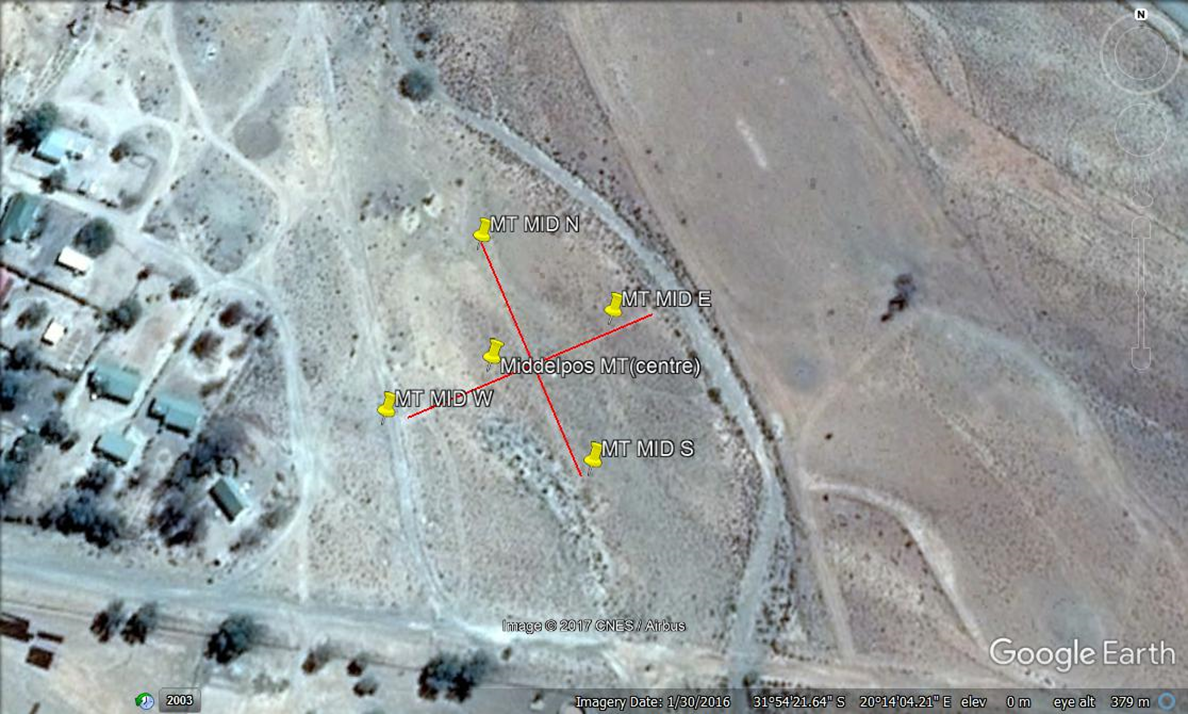
\includegraphics[width=\textwidth]{figures/site.png}
  \caption{Layout of the MT instrumentation at Middelpos. MID N(orth), MID S(south), MID E(ast), and MID W(est) indicate the locations of the electric field electrodes. The length of each electrode line is $100$~m. The LEMI-417 instrument is located at the crossing of the two electrode lines. The magnetometer is positioned $5$~m from the LEMI-417 to reduce the impact of the instrument currents on the magnetometer measurements. 
}
 \label{fig:site}
\end{figure}

The time series of 1--second--cadence electric, $\mathbf{E}(t)$, and magnetic, $\mathbf{B}(t)$, field measurements is shown in Figure~\ref{fig:timeseries}. Each component $k=x, y$ of $\mathbf{E}(t)$ was despiked by finding times when $|E_k(t+1)-E_k(t)|\ge 0.1$~mV/km and replacing values in the time range $[t-1, t+5]$ with linearly interpolated values based on $E_k(t-2)$ and $E_k(t+6)$. The number of spikes in $E_x(t)$ was $X$ \todo{insert value} ($X$\%) \todo{insert value}; for $E_y(t)$, the number was $X$ ($X$\%).

The averaged amplitudes of the Fourier coefficients for each vector component of the time series shown in Figure~\ref{fig:timeseries}(a) are shown in Figure~\ref{fig:timeseries}(b). The averaged amplitudes shown are frequency--domain averages of the discrete Fourier transform amplitudes. The values of the band centers, marked with filled circles, the number of values in each band, and the band boundaries are given in Tables~\ref{table:evalfreqs1d} and~\ref{table:evalfreqs119d} of Appendix~\ref{appendix:tables}. The vertical bars correspond to 95\% confidence intervals; the length of the confidence interval for the magnitude of a Fourier coefficient, $\Delta|\widetilde{A}|$, calculated using propagation of errors in $|\widetilde{A}| = \sqrt{A_r^2 + A_i^2}$, is

\begin{equation}
\Delta\big|\widetilde{A}\big| = \sqrt{(A_r\Delta A_r)^2 + (A_i\Delta A_i)^2} / \big|\widetilde{A}\big|
\end{equation}

\noindent
where $\Delta A_r$ and $\Delta A_i$ are the lengths of the 95\% confidence intervals for the real ($A_r$) and imaginary ($A_i$) parts of $\widetilde{A}$, respectively; $\widetilde{A}$ is one of the $\widetilde{B}_x$, $\widetilde{B}_y$, $\widetilde{E}_x$, and $\widetilde{E}_y$, which are frequency domain averages shown in Figure~\ref{fig:timeseries}(b). The lengths of the 95\% symmetric confidence intervals for the averages $A_r$ and $A_i$ were determined using $\pm 2 (s/\sqrt{n})t^{-1}_{n-1}(0.025)$, where $n$ is the number of values used to calculate the average, $t^{-1}_{n-1}(0.025)$ is the inverse $t$-distribution evaluated at $0.025$ and $s$ is the standard deviation of the sample.

\begin{figure}
     \subfigure[]{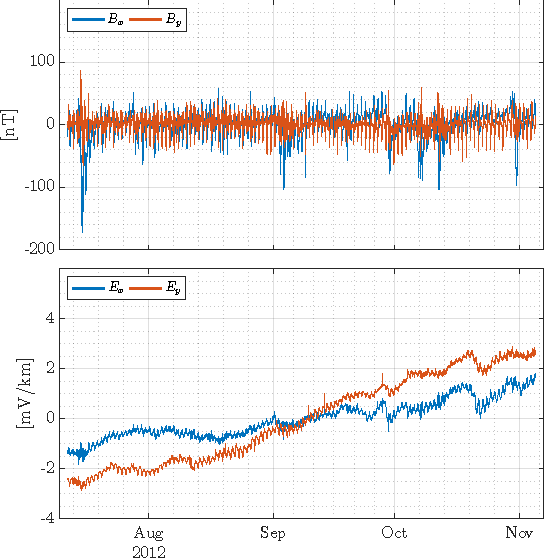
\includegraphics[width=0.45\textwidth]{figures/tsplot-original-Middelpos-tf1.pdf}}
     \hspace{10pt}
     \subfigure[]{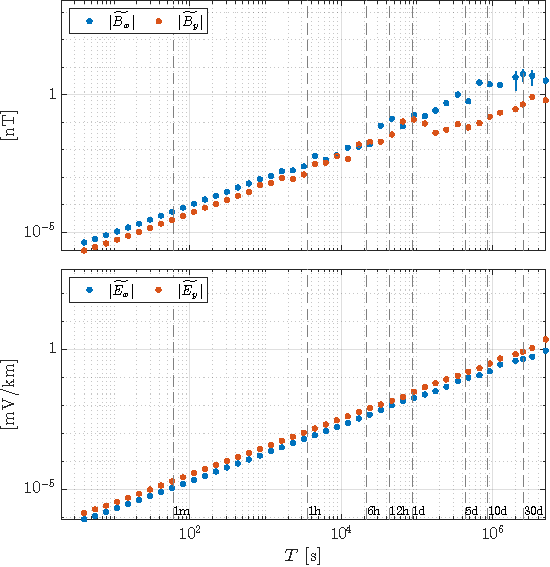
\includegraphics[width=0.45\textwidth]{figures/dftplot-original-averaged-magnitudes-Middelpos-tf1.pdf}}
     \caption{(a) Measurements used for analysis after mean subtraction and despiking. (b) Magnitudes of discrete Fourier transform coefficients for measurements in (a).}
  \label{fig:timeseries}
\end{figure}

\section{Models and Methods}
\label{section:Models_and_Methods}

$\mathbf{E}(t)$ and $\mathbf{B}(t)$ measurements are used to estimate the complex--valued transfer function matrix $\boldsymbol{\mathcal{\widetilde{Z}}}$ in

\begin{linenomath*}
    \begin{equation}
        \mathbf{\widetilde{E}}(f_e) = \boldsymbol{\mathcal{
    \widetilde{Z}}}(f_e)\mathbf{\widetilde{B}}(f_e)\text{ ,}
    \end{equation}
\end{linenomath*}

\noindent where $f_e$ is an ``evaluation frequency" and

\begin{linenomath*}
    \begin{equation}
        \boldsymbol{\mathcal{\widetilde{Z}}}(f_e) = 
            \begin{bmatrix}
                \widetilde{Z}_{xx}(f_e) & \widetilde{Z}_{xy}(f_e)\\
                \widetilde{Z}_{yx}(f_e) & \widetilde{Z}_{yy}(f_e)
            \end{bmatrix}
    \end{equation}
\end{linenomath*}

\noindent using a method described by \citeay{Sims1971}: for each $\mathbf{\widetilde{E}}$ vector component $k=x,y$, a four parameter over--determined linear regression is performed using

\begin{equation}
\widetilde{E}_k(f) = \widetilde{Z}_{kx}(f)\widetilde{B}_x(f) + \widetilde{Z}_{ky}(f)\widetilde{B}_y(f)
\label{eqn:single}
\end{equation}

\noindent with values of $f$ in a band around $f_e$. (The number of parameters is four because the two regression parameters $\widetilde{Z}_{kx}$ and $\widetilde{Z}_{ky}$ in Equation~\ref{eqn:single} are complex--valued; the actual regression is performed using only real numbers -- see \cite{Egbert1986}).

Two methods have been used for computing the Fourier coefficients -- one uses the standard DFT (Discrete Fourier Transform) formula for equally spaced records, typically implemented using the FFT algorithm. The other is an approximation based on the method of ``Cascade Decimation" \citep{Wight1980}, which can require less memory and produce logarithmically spaced evaluation frequencies. Here, we use the standard DFT formula because it is not an approximation.

There are two general methods for computing estimates of $\widetilde{Z}_{kx}$ and $\widetilde{Z}_{ky}$ for each evaluation frequency: (1) compute the Fourier coefficients using the full time series and then perform regression using the Fourier coefficients in a band centered on the evaluation frequency and (2) split the full time series into (possibly overlapping) segments, perform a regression on each segment using the Fourier coefficients in a band centered on the evaluation frequency to find segment estimates of $\widetilde{Z}_{kx}$ and $\widetilde{Z}_{ky}$, and then average the segment estimates of $\widetilde{Z}_{kx}$ and $\widetilde{Z}_{ky}$. In this paper, we present results from both methods; for the second method, non--overlapping time series segments were used, and the estimates of $\widetilde{Z}_{kx}$ and $\widetilde{Z}_{ky}$ are unweighted averages. 

There are two common modifications to these estimation methods. The first is the ``remote reference"  method, which involves using $\mathbf{B}(t)$ measurements covering the same time interval from a nearby magnetometer~\citep{Simpson2005}. In our case, we do not have such data. The second uses a robust algorithm for regression, which involves computing estimates of $\widetilde{Z}_{kx}$ and $\widetilde{Z}_{ky}$ using a custom error function instead of the standard sum--of--squares error function (\cite{Simpson2005}; see also~\cite{Thomson2016} for a discussion about the ``overselling'' of this method). The custom error function automatically downweights outliers. For the data considered, we have found that this method produces differing results only at evaluation frequencies where the signal-to-prediction error is less than 1.0.

\section{Results}
\label{section:Results}

Figure~\ref{fig:z} shows the results of the regression described in Section~\ref{section:Models_and_Methods}. For the components of $\boldsymbol{\mathcal{\widetilde{Z}}}$ computed using one $119$--day segment, 95\% confidence intervals were computed using formulas that assume the regression errors are independent and identically distributed (\cite{Draper1981}; chapter 2.6). For the magnitudes calculated using the average of $119$ one--day segments, the 95\% confidence intervals were calculated using the formula given in Section~\ref{section:Data} for the magnitudes of the DFT amplitudes. The error bars for the phases were calculated using propagation of errors on

$$\phi_{ij}=\tan^{-1}[\text{Im}(\widetilde{Z}_{ij})/\text{Re}(\widetilde{Z}_{ij})]$$

\noindent giving

$$\Delta\phi_{ij} = (1/|\widetilde{Z}_{ij}|^2) \sqrt{ \big[\text{Im}(\widetilde{Z}_{ij})\text{Re}(\Delta \widetilde{Z}_{ij})\big]^2 + \big[\text{Re}(\widetilde{Z}_{ij})\text{Im}(\Delta \widetilde{Z}_{ij}) \big]^2}.$$

\noindent where $\Delta \widetilde{Z}_{ij}$ is the 95\% confidence interval length for element $\widetilde{Z}_{ij}$ of $\boldsymbol{\mathcal{\widetilde{Z}}}$, $|\boldsymbol{\cdotp}|$ is the complex magnitude, and $\text{Re}(\boldsymbol{\cdotp})$ and $\text{Im}(\boldsymbol{\cdotp})$ are the real and imaginary parts of the argument, respectively.


The signal--to--error ratio, $\text{SE}_k(f_e)$, for component $k=x,y$ of $\mathbf{E}$ was calculated using 

\begin{equation}
\text{SE}_k(f_e) = \frac{\displaystyle\sum_{j=1}^{N_e} \left|\widetilde{E}_k(f_j)\right|^2}{\displaystyle\sum_{j=1}^{N_e}\left|\Delta\widetilde{E}_k(f_j)\right|^2}
\end{equation}

\noindent where $j$ is the index of the DFT frequency in the band centered on $f_e=1/T_e$; Tables~\ref{table:evalfreqs1d} and~\ref{table:evalfreqs119d} in Appendix~\ref{appendix:tables} list the band centers, ranges, and number of frequencies, $N_e$ in each band for each regression method. The error, $\Delta\widetilde{E}_k = \widetilde{E}_k^{\text{p}}-\widetilde{E}_k$, is the difference between the complex--valued DFT amplitudes of the predicted, $E_k^\text{p}(t)$, and measured, $E_k(t)$, signals after convolution with a Parzen window. The predicted signal, $E_k^{\text{p}}$, was computed by linearly interpolating the real and imaginary parts of $\widetilde{Z}_{kx}$ and $\widetilde{Z}_{ky}$ onto a uniform frequency grid of $N=86400\times 119$ points. At grid frequencies outside of the range of $f_e$ values, the interpolated values of $\widetilde{Z}_{kx}$ and $\widetilde{Z}_{ky}$ were set to zero. 95\% confidence intervals were computed using bootstrap resampling: at each $f_e$, the $N_e$ pairs of $\widetilde{Z}_{kx}$ and $\widetilde{Z}_{ky}$ were randomly selected with replacement, and the sums in the $\text{SE}$ formula were computed using these randomly selected pairs. This process was repeated $1,000$ times, and the results were sorted in ascending order; the maximum $\text{SE}$ error bar value is the $975$th value in the sorted list, and the minimum is the $25$th. No confidence intervals were computed if $N_e\le 10$.

The coherence, $\text{Coh}_{XY}(f_e)$, was computed using the 

\begin{equation}
\text{Coh}^2_{XY}(f_e) = \frac{\left|\displaystyle\sum_{j=1}^{N_e}\widetilde{X}^*(f_j)\widetilde{Y}(f_j)\right|^2}{\displaystyle\sum_{j=1}^{N_e} \left|\widetilde{X}(f_j)\right|^2\sum_{j=1}^{N_e} \left|\widetilde{Y}(f_j)\right|^2}
\end{equation}

\noindent where the summation frequencies and $f_e$ values are the same as those used for computing the $\text{SE}$. 95\% error bars were computed using the same as $\text{SE}$. The coherence was computed between the predicted field, $E^\text{p}_k(t)$, and the measured field, $E_k(t)$, and also between $E_x^\text{p}(t)$ and $B_y(t)$ and between $E_y^\text{p}(t)$ and $B_x(t)$.

Traditionally, the primary quality metric used for evaluating the transfer function is the $\text{Coh}^2_{E_xB_y}$ and $\text{Coh}^2_{E_yB_x}$. Here, we have also computed the coherences between the measured and predicted fields, $\text{Coh}^2_{E_kE^\text{p}_k}$ ($k=x,y$) as it is a more direct measure of the ability of the transfer function to reproduce the signal. Coherence has a limitation, however. Two signals that are identical except for a scaling factor will have the same coherence for any scaling factor. As a result, we have introduced the signal--to--error, which can be used to make a more direct assessment of how well the transfer function captures the measured signal.

Note that this differs from the exact signal--to--noise, $\text{Coh}^2/(1-\text{Coh}^2)$, which applies only if the input signal and the noise in the output signal (which is unknown) are uncorrelated and the input signal has no noise (\cite{Miranda2006}; \cite{Pedersen1988}).

%sxx = abs(sum(dftsegsx{s}.*conj(dftsegsx{s}),1));
%syy = abs(sum(dftsegsy{s}.*conj(dftsegsy{s}),1));
%sxy = abs(sum(conj(dftsegsx{s}).*dftsegsy{s},1));
%cxy(s,:) = sqrt(sxy/sqrt(sxx*syy));


\begin{figure}[h!]
  \vspace{-2em}
  \subfigure(a){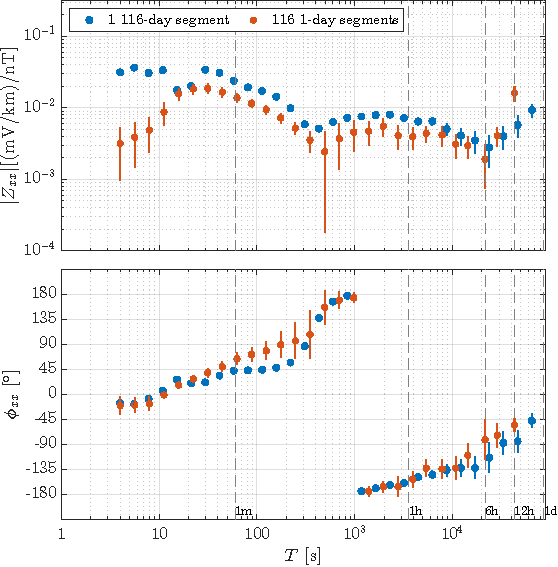
\includegraphics[width=0.48\textwidth]{figures/zplot-magnitude_phase-Middelpos-tf1;Middelpos-tf3-Z_xx.pdf}} 
  \subfigure(b){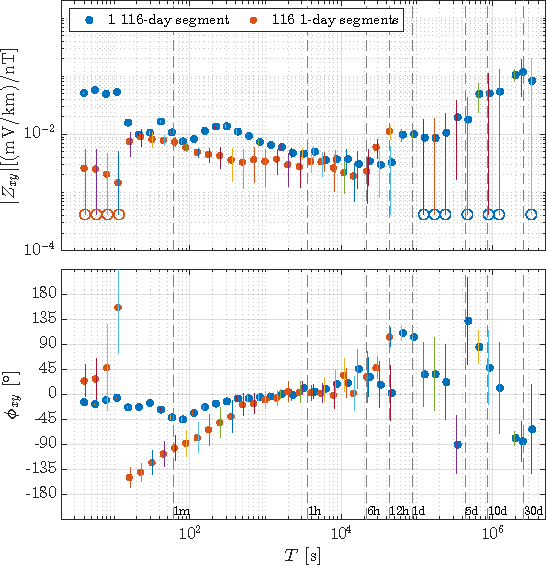
\includegraphics[width=0.48\textwidth]{figures/zplot-magnitude_phase-Middelpos-tf1;Middelpos-tf3-Z_xy.pdf}} 
  \subfigure(c){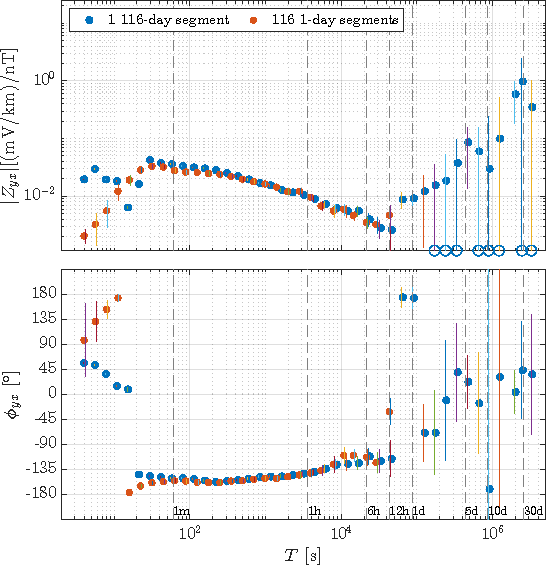
\includegraphics[width=0.48\textwidth]{figures/zplot-magnitude_phase-Middelpos-tf1;Middelpos-tf3-Z_yx.pdf}} 
  \subfigure(d){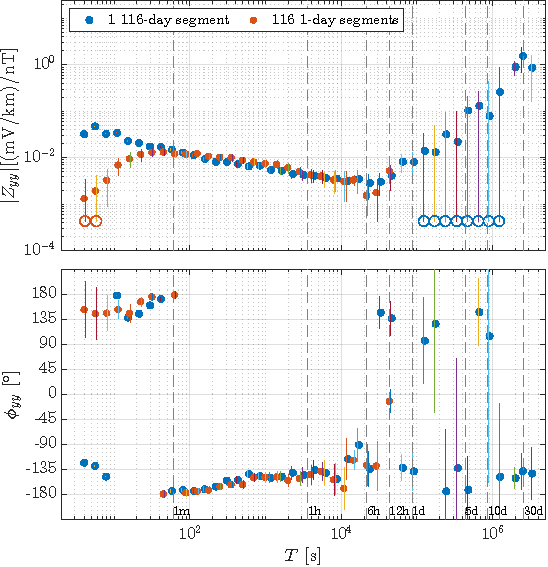
\includegraphics[width=0.48\textwidth]{figures/zplot-magnitude_phase-Middelpos-tf1;Middelpos-tf3-Z_yy.pdf}} 

  \caption{Magnitudes and phases for components of $\boldsymbol{\mathcal{\widetilde{Z}}}$: (a) $|\widetilde{Z}_{xx}|$ and $\phi_{xx}$; (b) $|\widetilde{Z}_{xy}|$ and $\phi_{xy}$; (c) $|\widetilde{Z}_{yx}|$ and $\phi_{yx}$; and (d) $|\widetilde{Z}_{yy}|$ and $\phi_{yy}$. Open circles on the lower part of the impedance amplitude error bars indicate that this formula yielded a value below zero. The gray background in plots shown in Figure~\ref{fig:z} corresponds to periods for which the signal-to-prediction error, shown in Figure~\ref{fig:se}, is greater than unity.}
  \label{fig:z}

  \subfigure(a){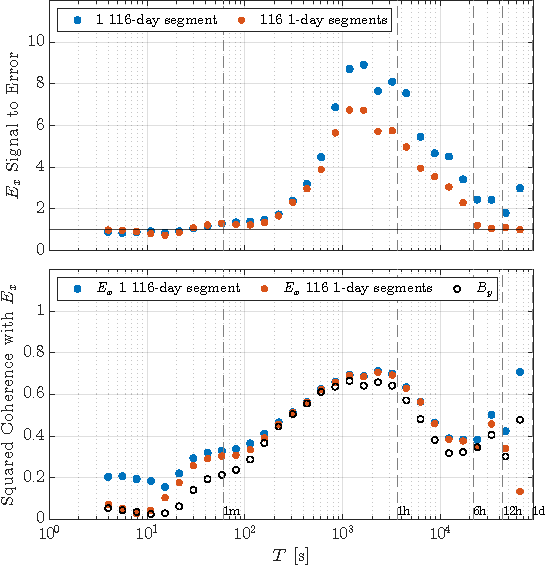
\includegraphics[width=0.48\textwidth]{figures/snplot-Middelpos-tf1;Middelpos-tf3-E_x.pdf}} 
  \subfigure(b){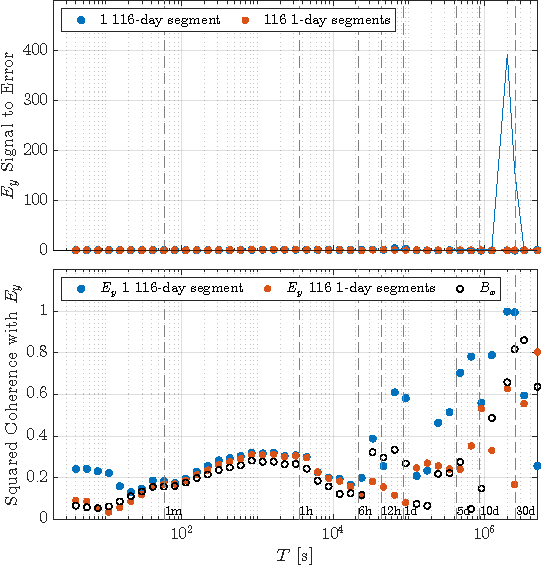
\includegraphics[width=0.48\textwidth]{figures/snplot-Middelpos-tf1;Middelpos-tf3-E_y.pdf}} 

  \caption{Model metrics for (a) $E_x$, which depends on $\widetilde{Z}_{xx}$ and $\widetilde{Z}_{xy}$ shown in Figure~\ref{fig:z}(a)-(b) and (b) $E_y$, which depends on $\widetilde{Z}_{yx}$ and $\widetilde{Z}_{yy}$ shown in  Figure~\ref{fig:z}(b)-(c).}
  \label{fig:se}

\end{figure}

%\begin{figure}[h!] 
%\end{figure}

\clearpage

\section{Comparision to KAP103}

\begin{figure}[h]
\centering
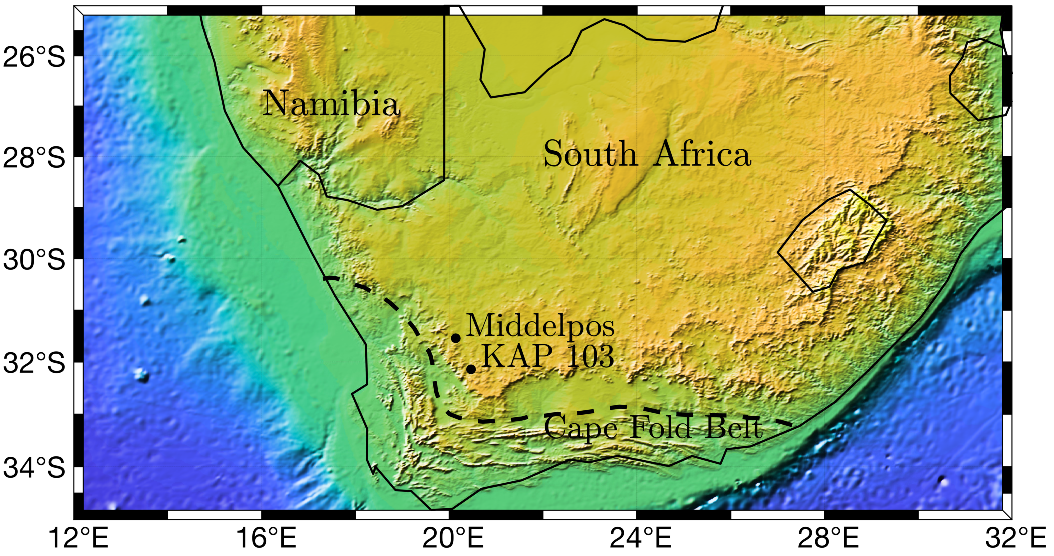
\includegraphics[width=\textwidth]{figures/map.pdf}
\caption{Location of Middelpos [$-31.906^\circ$, $20.234^\circ$] and KAP103 [$-32.139^\circ$, $20.468^\circ$] MT stations. The relief map is from the ETOPO1 Global Relief Model (\cite{NCEI2006}), and the Cape Fold Belt line was derived from the digitization of Figure~1 of \cite{Nguuri2001}}.
\label{fig:map}
\end{figure}

\begin{figure}[h]
     \subfigure[]{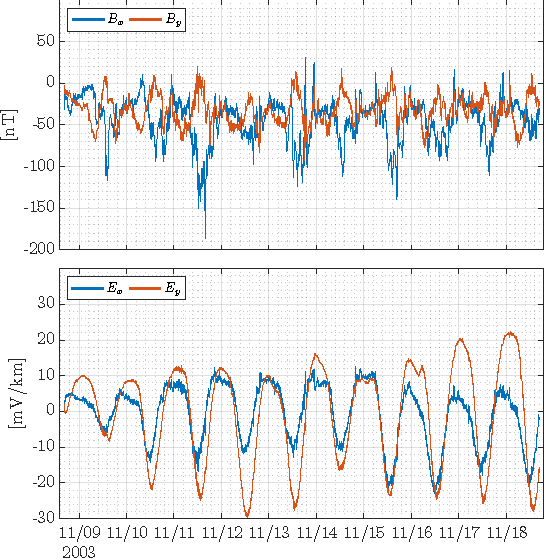
\includegraphics[width=0.45\textwidth]{figures/tsplot-original-KAP103-tf1.pdf}}
     \hspace{10pt}
     \subfigure[]{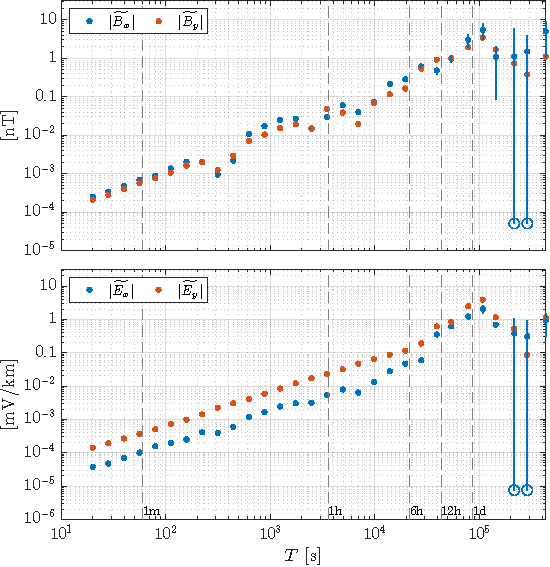
\includegraphics[width=0.45\textwidth]{figures/dftplot-original-averaged-magnitudes-KAP103-tf1.pdf}}
     \caption{(a) Measurements used for analysis after mean subtraction and despiking. (b) Magnitudes of discrete Fourier transform coefficients for measurements in (a).}
  \label{fig:timeseries}
\end{figure}

\clearpage

\section{Discussion}

\section{Appendix A}

\begin{figure}[h]
  \centering
  (a)
  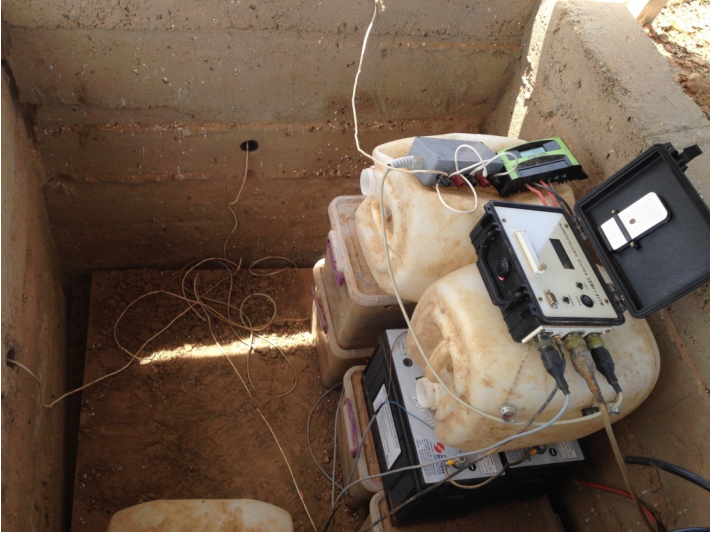
\includegraphics[width=0.45\textwidth]{figures/instrument.pdf}
  (b)
  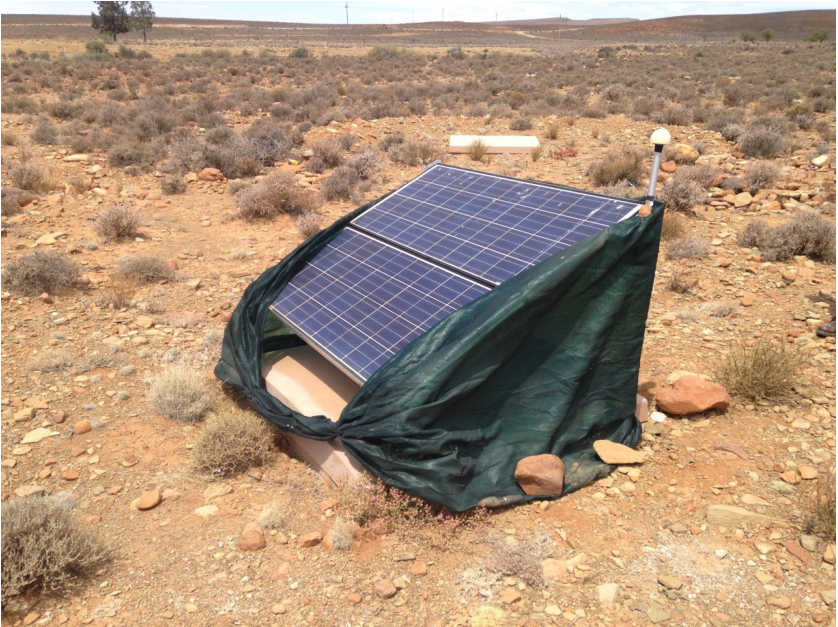
\includegraphics[width=0.45\textwidth]{figures/solarpanel.pdf}
  \caption{The Middelpos MT instrument. (a) The LEMI-417 instrument and the 12V lead-acid batteries that power it are in a subterranean enclosure with concrete walls. The instrument is mounted on two 25-liter water bottles to reduce temperature variation. (b) The solar panels are mounted on a steel frame over the enclosure. The side openings are covered with a canvas to prevent direct sunlight on the instrument. The small white dome above the solar panels is the GPS antenna.}
  \label{fig:lemi}
\end{figure}


\clearpage
\section{Appendix B}
\label{appendix:tables}

\begin{table}
  \caption{Evaluation frequencies, $f_e$, and periods, $T_e$, associated with evaluation frequency bands used for regression and spectra averaging using one--day segments. Subscript $l$ indicates a lower band bound and subscript $u$ an upper band bound. $i_l$ and $i_h$ are the lower and upper DFT frequency numbers, and $N_e$ is the number of DFT points in the band. $T=1/f$ and $i=1/86400$ for all subscripts.}
  \centering
  \small
\begin{tabular}{c c c c c c c c c}
\hline
$f_e$ [Hz] & $f_l$ [Hz] & $f_u$ [Hz] & $T_e$ [s] & $T_l$ [s] & $T_u$ [s] & $i_l$ & $i_u$ & $N_e$ \\
\hline
$2.31\cdot 10^{-5}$ & $1.16\cdot 10^{-5}$ & $3.47\cdot 10^{-5}$ & $4.32\cdot 10^{4}$ & $2.88\cdot 10^{4}$ & $8.64\cdot 10^{4}$ & $         2$ & $         4$ & $      3$\\
$3.47\cdot 10^{-5}$ & $2.31\cdot 10^{-5}$ & $4.63\cdot 10^{-5}$ & $2.88\cdot 10^{4}$ & $2.16\cdot 10^{4}$ & $4.32\cdot 10^{4}$ & $         3$ & $         5$ & $      3$\\
$4.63\cdot 10^{-5}$ & $3.47\cdot 10^{-5}$ & $5.79\cdot 10^{-5}$ & $2.16\cdot 10^{4}$ & $1.73\cdot 10^{4}$ & $2.88\cdot 10^{4}$ & $         4$ & $         6$ & $      3$\\
$6.94\cdot 10^{-5}$ & $4.63\cdot 10^{-5}$ & $9.26\cdot 10^{-5}$ & $1.44\cdot 10^{4}$ & $1.08\cdot 10^{4}$ & $2.16\cdot 10^{4}$ & $         5$ & $         9$ & $      5$\\
$9.26\cdot 10^{-5}$ & $6.94\cdot 10^{-5}$ & $1.16\cdot 10^{-4}$ & $1.08\cdot 10^{4}$ & $8.64\cdot 10^{3}$ & $1.44\cdot 10^{4}$ & $         7$ & $        11$ & $      5$\\
$1.27\cdot 10^{-4}$ & $9.26\cdot 10^{-5}$ & $1.62\cdot 10^{-4}$ & $7.85\cdot 10^{3}$ & $6.17\cdot 10^{3}$ & $1.08\cdot 10^{4}$ & $         9$ & $        15$ & $      7$\\
$1.85\cdot 10^{-4}$ & $1.27\cdot 10^{-4}$ & $2.43\cdot 10^{-4}$ & $5.40\cdot 10^{3}$ & $4.11\cdot 10^{3}$ & $7.85\cdot 10^{3}$ & $        12$ & $        22$ & $     11$\\
$2.55\cdot 10^{-4}$ & $1.85\cdot 10^{-4}$ & $3.24\cdot 10^{-4}$ & $3.93\cdot 10^{3}$ & $3.09\cdot 10^{3}$ & $5.40\cdot 10^{3}$ & $        17$ & $        29$ & $     13$\\
$3.59\cdot 10^{-4}$ & $2.55\cdot 10^{-4}$ & $4.63\cdot 10^{-4}$ & $2.79\cdot 10^{3}$ & $2.16\cdot 10^{3}$ & $3.93\cdot 10^{3}$ & $        23$ & $        41$ & $     19$\\
$5.09\cdot 10^{-4}$ & $3.59\cdot 10^{-4}$ & $6.60\cdot 10^{-4}$ & $1.96\cdot 10^{3}$ & $1.52\cdot 10^{3}$ & $2.79\cdot 10^{3}$ & $        32$ & $        58$ & $     27$\\
$7.18\cdot 10^{-4}$ & $5.09\cdot 10^{-4}$ & $9.26\cdot 10^{-4}$ & $1.39\cdot 10^{3}$ & $1.08\cdot 10^{3}$ & $1.96\cdot 10^{3}$ & $        45$ & $        81$ & $     37$\\
$1.02\cdot 10^{-3}$ & $7.18\cdot 10^{-4}$ & $1.32\cdot 10^{-3}$ & $9.82\cdot 10^{2}$ & $7.58\cdot 10^{2}$ & $1.39\cdot 10^{3}$ & $        63$ & $       115$ & $     53$\\
$1.44\cdot 10^{-3}$ & $1.02\cdot 10^{-3}$ & $1.85\cdot 10^{-3}$ & $6.97\cdot 10^{2}$ & $5.40\cdot 10^{2}$ & $9.82\cdot 10^{2}$ & $        89$ & $       161$ & $     73$\\
$2.03\cdot 10^{-3}$ & $1.44\cdot 10^{-3}$ & $2.62\cdot 10^{-3}$ & $4.94\cdot 10^{2}$ & $3.82\cdot 10^{2}$ & $6.97\cdot 10^{2}$ & $       125$ & $       227$ & $    103$\\
$2.86\cdot 10^{-3}$ & $2.03\cdot 10^{-3}$ & $3.69\cdot 10^{-3}$ & $3.50\cdot 10^{2}$ & $2.71\cdot 10^{2}$ & $4.94\cdot 10^{2}$ & $       176$ & $       320$ & $    145$\\
$4.03\cdot 10^{-3}$ & $2.86\cdot 10^{-3}$ & $5.20\cdot 10^{-3}$ & $2.48\cdot 10^{2}$ & $1.92\cdot 10^{2}$ & $3.50\cdot 10^{2}$ & $       248$ & $       450$ & $    203$\\
$5.68\cdot 10^{-3}$ & $4.03\cdot 10^{-3}$ & $7.34\cdot 10^{-3}$ & $1.76\cdot 10^{2}$ & $1.36\cdot 10^{2}$ & $2.48\cdot 10^{2}$ & $       349$ & $       635$ & $    287$\\
$8.02\cdot 10^{-3}$ & $5.68\cdot 10^{-3}$ & $1.04\cdot 10^{-2}$ & $1.25\cdot 10^{2}$ & $9.65\cdot 10^{1}$ & $1.76\cdot 10^{2}$ & $       492$ & $       896$ & $    405$\\
$1.13\cdot 10^{-2}$ & $8.02\cdot 10^{-3}$ & $1.46\cdot 10^{-2}$ & $8.84\cdot 10^{1}$ & $6.85\cdot 10^{1}$ & $1.25\cdot 10^{2}$ & $       694$ & $      1262$ & $    569$\\
$1.59\cdot 10^{-2}$ & $1.13\cdot 10^{-2}$ & $2.06\cdot 10^{-2}$ & $6.27\cdot 10^{1}$ & $4.86\cdot 10^{1}$ & $8.84\cdot 10^{1}$ & $       978$ & $      1780$ & $    803$\\
$2.25\cdot 10^{-2}$ & $1.59\cdot 10^{-2}$ & $2.91\cdot 10^{-2}$ & $4.44\cdot 10^{1}$ & $3.44\cdot 10^{1}$ & $6.27\cdot 10^{1}$ & $      1379$ & $      2511$ & $   1133$\\
$3.17\cdot 10^{-2}$ & $2.25\cdot 10^{-2}$ & $4.10\cdot 10^{-2}$ & $3.15\cdot 10^{1}$ & $2.44\cdot 10^{1}$ & $4.44\cdot 10^{1}$ & $      1945$ & $      3541$ & $   1597$\\
$4.48\cdot 10^{-2}$ & $3.17\cdot 10^{-2}$ & $5.78\cdot 10^{-2}$ & $2.23\cdot 10^{1}$ & $1.73\cdot 10^{1}$ & $3.15\cdot 10^{1}$ & $      2743$ & $      4995$ & $   2253$\\
$6.31\cdot 10^{-2}$ & $4.48\cdot 10^{-2}$ & $8.15\cdot 10^{-2}$ & $1.58\cdot 10^{1}$ & $1.23\cdot 10^{1}$ & $2.23\cdot 10^{1}$ & $      3869$ & $      7045$ & $   3177$\\
$8.91\cdot 10^{-2}$ & $6.31\cdot 10^{-2}$ & $1.15\cdot 10^{-1}$ & $1.12\cdot 10^{1}$ & $8.69\cdot 10^{0}$ & $1.58\cdot 10^{1}$ & $      5457$ & $      9939$ & $   4483$\\
$1.26\cdot 10^{-1}$ & $8.91\cdot 10^{-2}$ & $1.62\cdot 10^{-1}$ & $7.96\cdot 10^{0}$ & $6.16\cdot 10^{0}$ & $1.12\cdot 10^{1}$ & $      7698$ & $     14016$ & $   6319$\\
$1.77\cdot 10^{-1}$ & $1.26\cdot 10^{-1}$ & $2.29\cdot 10^{-1}$ & $5.64\cdot 10^{0}$ & $4.37\cdot 10^{0}$ & $7.96\cdot 10^{0}$ & $     10857$ & $     19771$ & $   8915$\\
$2.50\cdot 10^{-1}$ & $1.77\cdot 10^{-1}$ & $3.23\cdot 10^{-1}$ & $4.00\cdot 10^{0}$ & $3.10\cdot 10^{0}$ & $5.64\cdot 10^{0}$ & $     15314$ & $     27888$ & $  12575$\\
\hline \\
\end{tabular}
\label{table:evalfreqs1d}
\end{table}

\clearpage

\begin{table}
  \caption{Same as Figure~\ref{table:evalfreqs1d} except for the regression and spectra averaging for one 119--day segment and $i=1/(86400\cdot 119)=1/(10,281,600)$.}
  \centering
  \small
\begin{tabular}{c c c c c c c c c}
\hline
$f_e$ [Hz] & $f_l$ [Hz] & $f_u$ [Hz] & $T_e$ [s] & $T_l$ [s] & $T_u$ [s] & $i_l$ & $i_u$ & $N_e$ \\
\hline
$1.95\cdot 10^{-7}$ & $9.73\cdot 10^{-8}$ & $2.92\cdot 10^{-7}$ & $5.14\cdot 10^{6}$ & $3.43\cdot 10^{6}$ & $1.03\cdot 10^{7}$ & $         2$ & $         4$ & $      3$\\
$2.92\cdot 10^{-7}$ & $1.95\cdot 10^{-7}$ & $3.89\cdot 10^{-7}$ & $3.43\cdot 10^{6}$ & $2.57\cdot 10^{6}$ & $5.14\cdot 10^{6}$ & $         3$ & $         5$ & $      3$\\
$3.89\cdot 10^{-7}$ & $2.92\cdot 10^{-7}$ & $4.86\cdot 10^{-7}$ & $2.57\cdot 10^{6}$ & $2.06\cdot 10^{6}$ & $3.43\cdot 10^{6}$ & $         4$ & $         6$ & $      3$\\
$4.86\cdot 10^{-7}$ & $3.89\cdot 10^{-7}$ & $5.84\cdot 10^{-7}$ & $2.06\cdot 10^{6}$ & $1.71\cdot 10^{6}$ & $2.57\cdot 10^{6}$ & $         5$ & $         7$ & $      3$\\
$7.78\cdot 10^{-7}$ & $4.86\cdot 10^{-7}$ & $1.07\cdot 10^{-6}$ & $1.29\cdot 10^{6}$ & $9.35\cdot 10^{5}$ & $2.06\cdot 10^{6}$ & $         6$ & $        12$ & $      7$\\
$1.07\cdot 10^{-6}$ & $7.78\cdot 10^{-7}$ & $1.36\cdot 10^{-6}$ & $9.35\cdot 10^{5}$ & $7.34\cdot 10^{5}$ & $1.29\cdot 10^{6}$ & $         9$ & $        15$ & $      7$\\
$1.46\cdot 10^{-6}$ & $1.07\cdot 10^{-6}$ & $1.85\cdot 10^{-6}$ & $6.85\cdot 10^{5}$ & $5.41\cdot 10^{5}$ & $9.35\cdot 10^{5}$ & $        12$ & $        20$ & $      9$\\
$2.04\cdot 10^{-6}$ & $1.46\cdot 10^{-6}$ & $2.63\cdot 10^{-6}$ & $4.90\cdot 10^{5}$ & $3.81\cdot 10^{5}$ & $6.85\cdot 10^{5}$ & $        16$ & $        28$ & $     13$\\
$2.82\cdot 10^{-6}$ & $2.04\cdot 10^{-6}$ & $3.60\cdot 10^{-6}$ & $3.55\cdot 10^{5}$ & $2.78\cdot 10^{5}$ & $4.90\cdot 10^{5}$ & $        22$ & $        38$ & $     17$\\
$3.99\cdot 10^{-6}$ & $2.82\cdot 10^{-6}$ & $5.15\cdot 10^{-6}$ & $2.51\cdot 10^{5}$ & $1.94\cdot 10^{5}$ & $3.55\cdot 10^{5}$ & $        30$ & $        54$ & $     25$\\
$5.54\cdot 10^{-6}$ & $3.99\cdot 10^{-6}$ & $7.10\cdot 10^{-6}$ & $1.80\cdot 10^{5}$ & $1.41\cdot 10^{5}$ & $2.51\cdot 10^{5}$ & $        42$ & $        74$ & $     33$\\
$7.78\cdot 10^{-6}$ & $5.54\cdot 10^{-6}$ & $1.00\cdot 10^{-5}$ & $1.29\cdot 10^{5}$ & $9.98\cdot 10^{4}$ & $1.80\cdot 10^{5}$ & $        58$ & $       104$ & $     47$\\
$1.08\cdot 10^{-5}$ & $7.78\cdot 10^{-6}$ & $1.38\cdot 10^{-5}$ & $9.26\cdot 10^{4}$ & $7.24\cdot 10^{4}$ & $1.29\cdot 10^{5}$ & $        81$ & $       143$ & $     63$\\
$1.52\cdot 10^{-5}$ & $1.08\cdot 10^{-5}$ & $1.95\cdot 10^{-5}$ & $6.59\cdot 10^{4}$ & $5.12\cdot 10^{4}$ & $9.26\cdot 10^{4}$ & $       112$ & $       202$ & $     91$\\
$2.11\cdot 10^{-5}$ & $1.52\cdot 10^{-5}$ & $2.70\cdot 10^{-5}$ & $4.74\cdot 10^{4}$ & $3.70\cdot 10^{4}$ & $6.59\cdot 10^{4}$ & $       157$ & $       279$ & $    123$\\
$2.96\cdot 10^{-5}$ & $2.11\cdot 10^{-5}$ & $3.80\cdot 10^{-5}$ & $3.38\cdot 10^{4}$ & $2.63\cdot 10^{4}$ & $4.74\cdot 10^{4}$ & $       218$ & $       392$ & $    175$\\
$4.13\cdot 10^{-5}$ & $2.96\cdot 10^{-5}$ & $5.31\cdot 10^{-5}$ & $2.42\cdot 10^{4}$ & $1.88\cdot 10^{4}$ & $3.38\cdot 10^{4}$ & $       305$ & $       547$ & $    243$\\
$5.78\cdot 10^{-5}$ & $4.13\cdot 10^{-5}$ & $7.42\cdot 10^{-5}$ & $1.73\cdot 10^{4}$ & $1.35\cdot 10^{4}$ & $2.42\cdot 10^{4}$ & $       426$ & $       764$ & $    339$\\
$8.07\cdot 10^{-5}$ & $5.78\cdot 10^{-5}$ & $1.04\cdot 10^{-4}$ & $1.24\cdot 10^{4}$ & $9.65\cdot 10^{3}$ & $1.73\cdot 10^{4}$ & $       595$ & $      1067$ & $    473$\\
$1.13\cdot 10^{-4}$ & $8.07\cdot 10^{-5}$ & $1.45\cdot 10^{-4}$ & $8.86\cdot 10^{3}$ & $6.90\cdot 10^{3}$ & $1.24\cdot 10^{4}$ & $       831$ & $      1491$ & $    661$\\
$1.58\cdot 10^{-4}$ & $1.13\cdot 10^{-4}$ & $2.03\cdot 10^{-4}$ & $6.34\cdot 10^{3}$ & $4.93\cdot 10^{3}$ & $8.86\cdot 10^{3}$ & $      1161$ & $      2085$ & $    925$\\
$2.20\cdot 10^{-4}$ & $1.58\cdot 10^{-4}$ & $2.83\cdot 10^{-4}$ & $4.54\cdot 10^{3}$ & $3.53\cdot 10^{3}$ & $6.34\cdot 10^{3}$ & $      1623$ & $      2913$ & $   1291$\\
$3.08\cdot 10^{-4}$ & $2.20\cdot 10^{-4}$ & $3.96\cdot 10^{-4}$ & $3.24\cdot 10^{3}$ & $2.53\cdot 10^{3}$ & $4.54\cdot 10^{3}$ & $      2268$ & $      4072$ & $   1805$\\
$4.31\cdot 10^{-4}$ & $3.08\cdot 10^{-4}$ & $5.54\cdot 10^{-4}$ & $2.32\cdot 10^{3}$ & $1.81\cdot 10^{3}$ & $3.24\cdot 10^{3}$ & $      3170$ & $      5692$ & $   2523$\\
$6.02\cdot 10^{-4}$ & $4.31\cdot 10^{-4}$ & $7.74\cdot 10^{-4}$ & $1.66\cdot 10^{3}$ & $1.29\cdot 10^{3}$ & $2.32\cdot 10^{3}$ & $      4431$ & $      7957$ & $   3527$\\
$8.42\cdot 10^{-4}$ & $6.02\cdot 10^{-4}$ & $1.08\cdot 10^{-3}$ & $1.19\cdot 10^{3}$ & $9.25\cdot 10^{2}$ & $1.66\cdot 10^{3}$ & $      6194$ & $     11120$ & $   4927$\\
$1.18\cdot 10^{-3}$ & $8.42\cdot 10^{-4}$ & $1.51\cdot 10^{-3}$ & $8.50\cdot 10^{2}$ & $6.61\cdot 10^{2}$ & $1.19\cdot 10^{3}$ & $      8657$ & $     15545$ & $   6889$\\
$1.64\cdot 10^{-3}$ & $1.18\cdot 10^{-3}$ & $2.11\cdot 10^{-3}$ & $6.08\cdot 10^{2}$ & $4.73\cdot 10^{2}$ & $8.50\cdot 10^{2}$ & $     12101$ & $     21727$ & $   9627$\\
$2.30\cdot 10^{-3}$ & $1.64\cdot 10^{-3}$ & $2.95\cdot 10^{-3}$ & $4.35\cdot 10^{2}$ & $3.39\cdot 10^{2}$ & $6.08\cdot 10^{2}$ & $     16914$ & $     30372$ & $  13459$\\
$3.21\cdot 10^{-3}$ & $2.30\cdot 10^{-3}$ & $4.13\cdot 10^{-3}$ & $3.11\cdot 10^{2}$ & $2.42\cdot 10^{2}$ & $4.35\cdot 10^{2}$ & $     23643$ & $     42453$ & $  18811$\\
$4.49\cdot 10^{-3}$ & $3.21\cdot 10^{-3}$ & $5.77\cdot 10^{-3}$ & $2.23\cdot 10^{2}$ & $1.73\cdot 10^{2}$ & $3.11\cdot 10^{2}$ & $     33048$ & $     59340$ & $  26293$\\
$6.28\cdot 10^{-3}$ & $4.49\cdot 10^{-3}$ & $8.07\cdot 10^{-3}$ & $1.59\cdot 10^{2}$ & $1.24\cdot 10^{2}$ & $2.23\cdot 10^{2}$ & $     46194$ & $     82948$ & $  36755$\\
$8.78\cdot 10^{-3}$ & $6.28\cdot 10^{-3}$ & $1.13\cdot 10^{-2}$ & $1.14\cdot 10^{2}$ & $8.87\cdot 10^{1}$ & $1.59\cdot 10^{2}$ & $     64571$ & $    115947$ & $  51377$\\
$1.23\cdot 10^{-2}$ & $8.78\cdot 10^{-3}$ & $1.58\cdot 10^{-2}$ & $8.15\cdot 10^{1}$ & $6.34\cdot 10^{1}$ & $1.14\cdot 10^{2}$ & $     90259$ & $    162071$ & $  71813$\\
$1.72\cdot 10^{-2}$ & $1.23\cdot 10^{-2}$ & $2.20\cdot 10^{-2}$ & $5.83\cdot 10^{1}$ & $4.54\cdot 10^{1}$ & $8.15\cdot 10^{1}$ & $    126165$ & $    226547$ & $ 100383$\\
$2.40\cdot 10^{-2}$ & $1.72\cdot 10^{-2}$ & $3.08\cdot 10^{-2}$ & $4.17\cdot 10^{1}$ & $3.25\cdot 10^{1}$ & $5.83\cdot 10^{1}$ & $    176356$ & $    316670$ & $ 140315$\\
$3.35\cdot 10^{-2}$ & $2.40\cdot 10^{-2}$ & $4.31\cdot 10^{-2}$ & $2.98\cdot 10^{1}$ & $2.32\cdot 10^{1}$ & $4.17\cdot 10^{1}$ & $    246513$ & $    442649$ & $ 196137$\\
$4.68\cdot 10^{-2}$ & $3.35\cdot 10^{-2}$ & $6.02\cdot 10^{-2}$ & $2.13\cdot 10^{1}$ & $1.66\cdot 10^{1}$ & $2.98\cdot 10^{1}$ & $    344581$ & $    618745$ & $ 274165$\\
$6.55\cdot 10^{-2}$ & $4.68\cdot 10^{-2}$ & $8.41\cdot 10^{-2}$ & $1.53\cdot 10^{1}$ & $1.19\cdot 10^{1}$ & $2.13\cdot 10^{1}$ & $    481663$ & $    864893$ & $ 383231$\\
$9.15\cdot 10^{-2}$ & $6.55\cdot 10^{-2}$ & $1.18\cdot 10^{-1}$ & $1.09\cdot 10^{1}$ & $8.50\cdot 10^{0}$ & $1.53\cdot 10^{1}$ & $    673278$ & $   1208966$ & $ 535689$\\
$1.28\cdot 10^{-1}$ & $9.15\cdot 10^{-2}$ & $1.64\cdot 10^{-1}$ & $7.82\cdot 10^{0}$ & $6.08\cdot 10^{0}$ & $1.09\cdot 10^{1}$ & $    941122$ & $   1689920$ & $ 748799$\\
$1.79\cdot 10^{-1}$ & $1.28\cdot 10^{-1}$ & $2.30\cdot 10^{-1}$ & $5.59\cdot 10^{0}$ & $4.35\cdot 10^{0}$ & $7.82\cdot 10^{0}$ & $   1315521$ & $   2362205$ & $1046685$\\
$2.50\cdot 10^{-1}$ & $1.79\cdot 10^{-1}$ & $3.21\cdot 10^{-1}$ & $4.00\cdot 10^{0}$ & $3.11\cdot 10^{0}$ & $5.59\cdot 10^{0}$ & $   1838863$ & $   3301939$ & $1463077$\\
\hline \\
\end{tabular}
\label{table:evalfreqs119d}
\end{table}

\clearpage

\bibliography{main.bib}

\end{document}
